% Options for packages loaded elsewhere
\PassOptionsToPackage{unicode}{hyperref}
\PassOptionsToPackage{hyphens}{url}
%
\documentclass[
]{book}
\usepackage{lmodern}
\usepackage{amssymb,amsmath}
\usepackage{ifxetex,ifluatex}
\ifnum 0\ifxetex 1\fi\ifluatex 1\fi=0 % if pdftex
  \usepackage[T1]{fontenc}
  \usepackage[utf8]{inputenc}
  \usepackage{textcomp} % provide euro and other symbols
\else % if luatex or xetex
  \usepackage{unicode-math}
  \defaultfontfeatures{Scale=MatchLowercase}
  \defaultfontfeatures[\rmfamily]{Ligatures=TeX,Scale=1}
\fi
% Use upquote if available, for straight quotes in verbatim environments
\IfFileExists{upquote.sty}{\usepackage{upquote}}{}
\IfFileExists{microtype.sty}{% use microtype if available
  \usepackage[]{microtype}
  \UseMicrotypeSet[protrusion]{basicmath} % disable protrusion for tt fonts
}{}
\makeatletter
\@ifundefined{KOMAClassName}{% if non-KOMA class
  \IfFileExists{parskip.sty}{%
    \usepackage{parskip}
  }{% else
    \setlength{\parindent}{0pt}
    \setlength{\parskip}{6pt plus 2pt minus 1pt}}
}{% if KOMA class
  \KOMAoptions{parskip=half}}
\makeatother
\usepackage{xcolor}
\IfFileExists{xurl.sty}{\usepackage{xurl}}{} % add URL line breaks if available
\IfFileExists{bookmark.sty}{\usepackage{bookmark}}{\usepackage{hyperref}}
\hypersetup{
  pdftitle={ ``Ciência de Dados na Educação Pública: Relatório 2021.1''},
  pdfauthor={Equipe Ciência de Dados na Educação Pública},
  hidelinks,
  pdfcreator={LaTeX via pandoc}}
\urlstyle{same} % disable monospaced font for URLs
\usepackage{longtable,booktabs}
% Correct order of tables after \paragraph or \subparagraph
\usepackage{etoolbox}
\makeatletter
\patchcmd\longtable{\par}{\if@noskipsec\mbox{}\fi\par}{}{}
\makeatother
% Allow footnotes in longtable head/foot
\IfFileExists{footnotehyper.sty}{\usepackage{footnotehyper}}{\usepackage{footnote}}
\makesavenoteenv{longtable}
\usepackage{graphicx,grffile}
\makeatletter
\def\maxwidth{\ifdim\Gin@nat@width>\linewidth\linewidth\else\Gin@nat@width\fi}
\def\maxheight{\ifdim\Gin@nat@height>\textheight\textheight\else\Gin@nat@height\fi}
\makeatother
% Scale images if necessary, so that they will not overflow the page
% margins by default, and it is still possible to overwrite the defaults
% using explicit options in \includegraphics[width, height, ...]{}
\setkeys{Gin}{width=\maxwidth,height=\maxheight,keepaspectratio}
% Set default figure placement to htbp
\makeatletter
\def\fps@figure{htbp}
\makeatother
\setlength{\emergencystretch}{3em} % prevent overfull lines
\providecommand{\tightlist}{%
  \setlength{\itemsep}{0pt}\setlength{\parskip}{0pt}}
\setcounter{secnumdepth}{5}
\usepackage{booktabs}
\usepackage[]{natbib}
\bibliographystyle{apalike}

\title{
\includegraphics[width=0.25in,height=\textheight]{logo.png} ``Ciência de Dados na Educação Pública: Relatório 2021.1''}
\author{Equipe Ciência de Dados na Educação Pública}
\date{}

\begin{document}
\maketitle

{
\setcounter{tocdepth}{1}
\tableofcontents
}
\hypertarget{apresentauxe7uxe3o---relatuxf3rio-2020.1}{%
\chapter{Apresentação - Relatório 2020.1}\label{apresentauxe7uxe3o---relatuxf3rio-2020.1}}

O avanço do uso de informações para solucionar diferentes tipos de questões e problemas gerou muitas mudanças em um curto espaço de tempo na história da sociedade. Novos questionamentos e desafios surgem em um contexto marcado pela Tecnologia da Informação e Comunicação, orientada ou dominada por notícias falsas (fake news), por grandes massas de dados (Big data) e pela internet das coisas (Internet of things). O reconhecimento de problemas e oportunidades requer soluções e tomadas de decisões cada vez mais personalizadas, lançando mão dos avanços da ciência no sentido de contribuir para o incremento das formas de pensar e, com isso, para o impulso da qualidade de vida. Assim, algoritmos e tecnologias trazem na sua concepção também vieses sociais, raciais ou de gênero que beneficiam uma parte privilegiada da sociedade. Por isso, vem sendo preciso desenvolver mecanismos e oportunidades de apoio à formação de cidadãos para torná-los capazes, por exemplo, de entender como as empresas têm acesso aos seus dados, como são construídos modelos que preveem seus desejos e como algoritmos podem afetar suas decisões e seu senso crítico. Cidadãos que usem suas experiências para compreender o universo científico sob diferentes aspectos e com percepção da interdisciplinaridade de soluções de problemas cotidianos; com habilidades de exploração e abstração das diversas realidades e cenários que impactam diretamente ou tangencialmente o seu cotidiano e sua comunidade; com visões críticas ampliadas acerca da cidade e da sociedade, bem como se percebam e atuem como protagonistas de mudanças e transformações da sociedade e resilientes frente a um futuro incerto, agravado durante a pandemia.

\emph{``Não podemos inserir indivíduos menos privilegiados em uma~estrutura social que é originalmente codificada para os~privilegiados, temos que mudar a estrutura.''\\
Parafraseando Mary Beardy para Women \& Power: O Manifesto,~2017: ``You cannot easily fit women into a structure that is~already coded as male; you have to change the structure.''}

\hypertarget{objetivos}{%
\section*{Objetivos}\label{objetivos}}
\addcontentsline{toc}{section}{Objetivos}

O projeto Ciência de Dados na Educação Pública atua no desenvolvimento de ferramentas e meios para apoiar a formação de estudantes e a capacitação de professoras/es na área de ciência de dados de modo a reconhecerem, construírem e proporem soluções para problemas da sociedade.
Ampliando as ações do Projeto Meninas na Ciência de Dados, passa-se a abraçar toda comunidade escolar, estudantes do ensino fundamental II e médio, sem distinção de sexo.
A nova estratégia de ação, além de cotar com a liderança integrada entre as escolas, a universidade e a comunidade, fundamenta todo o material didático utilizado e em construção no cotidiano de vulnerabilidades sociais, raciais e de gênero, mas estende-se a outras escolas da rede pública, visando, assim, a construção de novos territórios educacionais.

\hypertarget{puxfablico-alvo}{%
\section*{Público Alvo}\label{puxfablico-alvo}}
\addcontentsline{toc}{section}{Público Alvo}

As ferramentas desenvolvidas visam beneficiar 1000 estudantes de cinco escolas públicas: Colégio Estadual Evaristo da Veiga (EV), Colégio Estadual Henriqueta Martins Catharino (HM), Colégio Estadual Ypiranga (YP), Colégio Estadual Mário Costa Neto (MC) e Escola Municipal Cidade de Jequié (CJ).
Através de uma parceria em construção com o Instituto Anísio Teixeira, trabalha-se para que todo o material desenvolvido e em desenvolvimento seja disponibilizado para toda a rede de ensino público (e privado).
Na Figura \ref{fig:estudcdnaep} é apresentada a equipe de estudantes bolsistas do projeto. Atualmente, em um contexto pandêmico, que dificulta o acesso a encontros on-line, 29 estudantes participam de modo frequente, mas este número triplicará com o retorno das atividades presenciais.

\begin{figure}
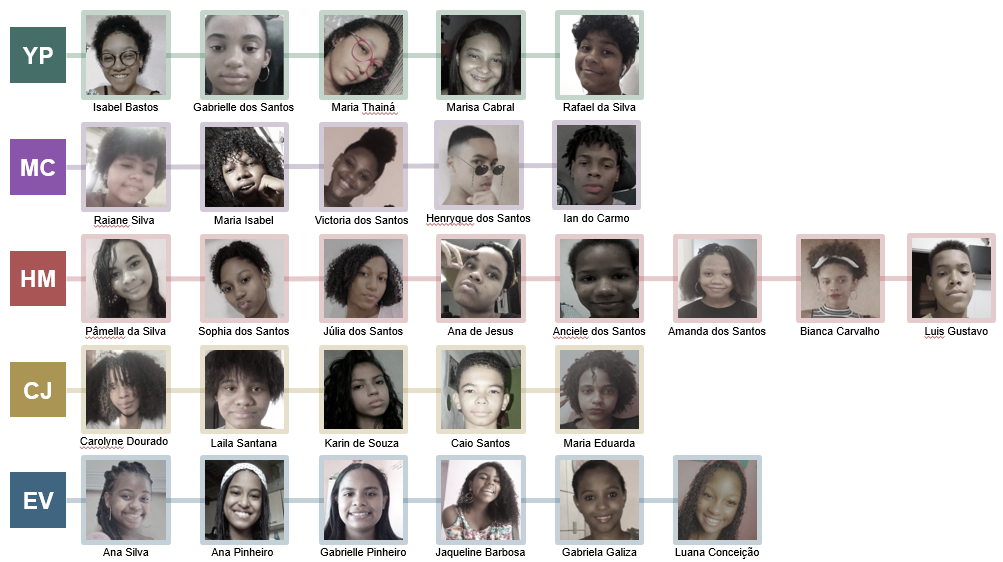
\includegraphics[width=13.93in]{images/image111} \caption{Equipe de estudantes bolsistas do projeto Ciência de Dados na Escola Pública}\label{fig:estudcdnaep}
\end{figure}

\hypertarget{equipe}{%
\section*{Equipe}\label{equipe}}
\addcontentsline{toc}{section}{Equipe}

Uma equipe multidisciplinar, composta por estudantes de graduação (5) e pós-graduação (7) e por professoras/es e profissionais que atuam em instituições de ensino superior se dividem em sete grupos de ação (ver Figura \ref{fig:profcdnaep}):

\begin{itemize}
\tightlist
\item
  Coordenação e Secretaria;
\item
  Ciência de Dados;
\item
  Inteligência Artificial;
\item
  Produção do Conhecimento Científico;
\item
  (re)Conhecendo Salvador;
\item
  Protagonismo;
\item
  Avaliação de Impactos do Projeto.
\end{itemize}

\begin{figure}
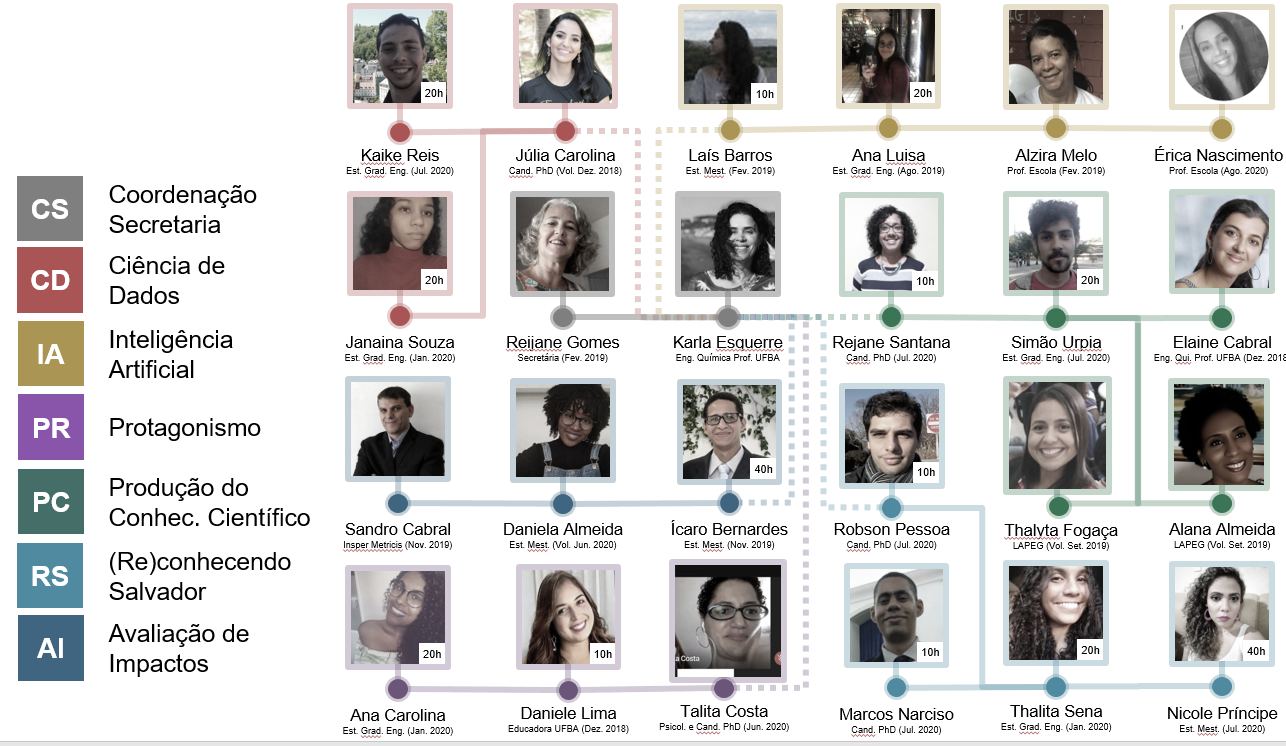
\includegraphics[width=17.86in]{images/image113} \caption{Equipe do projeto Ciência de Dados na Escola Pública}\label{fig:profcdnaep}
\end{figure}

\hypertarget{palavra-da-coordenadora}{%
\chapter*{Palavra da Coordenadora}\label{palavra-da-coordenadora}}
\addcontentsline{toc}{chapter}{Palavra da Coordenadora}

Texto de Karla

\hypertarget{resumo}{%
\chapter*{Resumo}\label{resumo}}
\addcontentsline{toc}{chapter}{Resumo}

Informações mais importantes, condensadas do relatório em texto com poucos parágrafos.

\hypertarget{contexto}{%
\chapter{Contexto}\label{contexto}}

Contextualização, referência a relatórios anteriores. Mais uma vez, importante ser sucinto por que há um relatório de 2019 extenso. A ideia é trazer as pessoas para o ponto imediatamente anterior ao período coberto pelo relatório (como uma retrospectiva).

\hypertarget{cafe}{%
\chapter{Café com Dados}\label{cafe}}

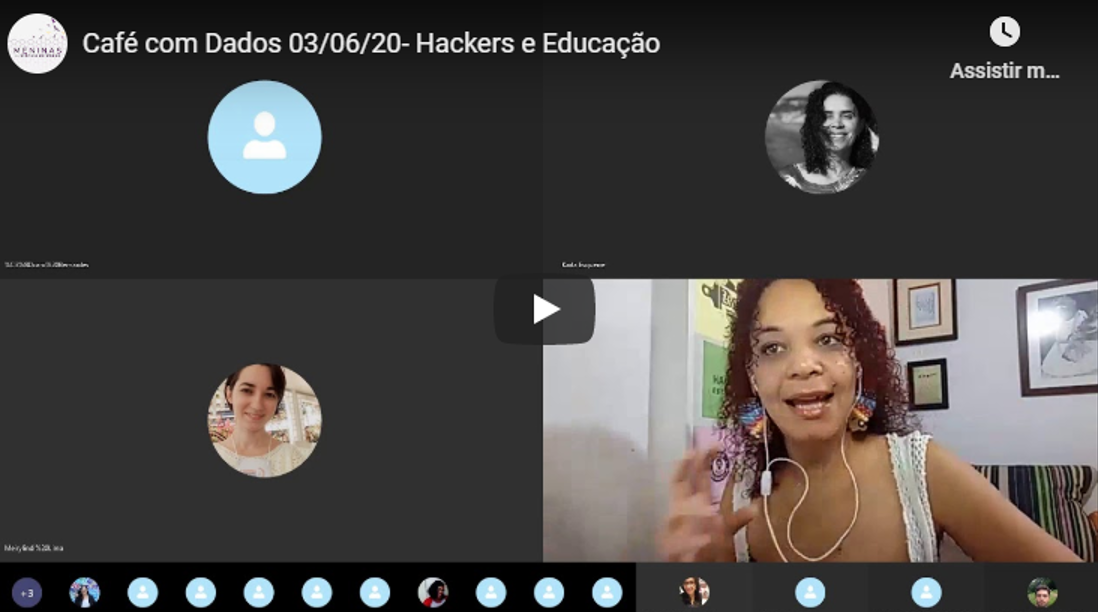
\includegraphics{cafe01.png}

Karina Menezes apresentando a cultura hackerista durante uma das sessões do Café com Dados

\leavevmode\hypertarget{resumo01}{}%
\textbf{Alvo:} Introduzir professores à Ciência de Dados

\leavevmode\hypertarget{resumo02}{}%
\textbf{Dificuldades:} Adesão dos professores, barulhos de fundo

\leavevmode\hypertarget{resumo03}{}%
\textbf{Soluções:} Consulta da opnião dos professores

\leavevmode\hypertarget{resumo04}{}%
\textbf{Resultados:} Ampliação do vocabulário dos professores?

\hypertarget{cafe_ativ}{%
\section{Apresentando a atividade}\label{cafe_ativ}}

\hypertarget{impactos}{%
\chapter{Avaliação de impactos}\label{impactos}}

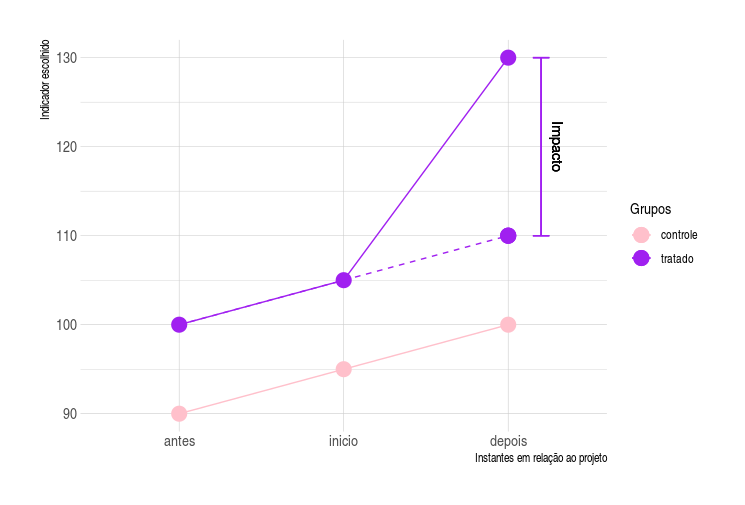
\includegraphics{impacto01.png}

Representação da avaliação de impacto

\hypertarget{notas-dos-estudantes}{%
\section{Notas dos estudantes}\label{notas-dos-estudantes}}

Impactos gerais, não alocados a uma atividade específica.

\hypertarget{respostas-de-questionuxe1rios}{%
\section{Respostas de questionários}\label{respostas-de-questionuxe1rios}}

\hypertarget{financeira}{%
\chapter{Execução financeira}\label{financeira}}

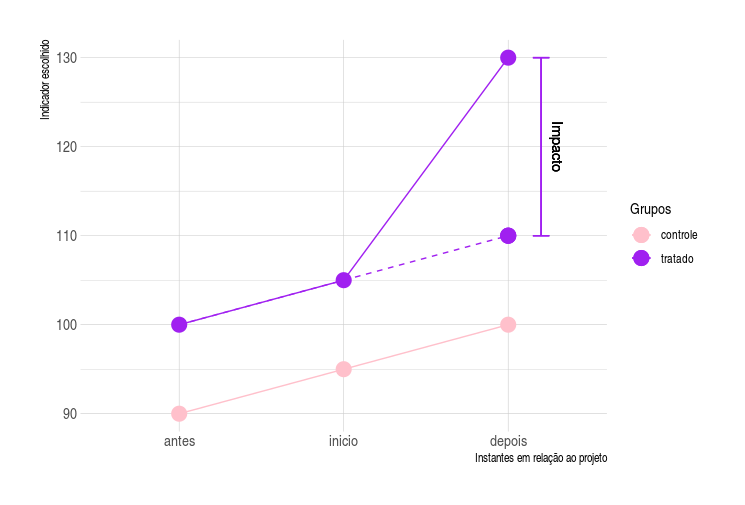
\includegraphics{impacto01.png}

Representação da avaliação de impacto

\hypertarget{detalhamento}{%
\section{Detalhamento}\label{detalhamento}}

\hypertarget{extras}{%
\chapter{Elementos extras}\label{extras}}

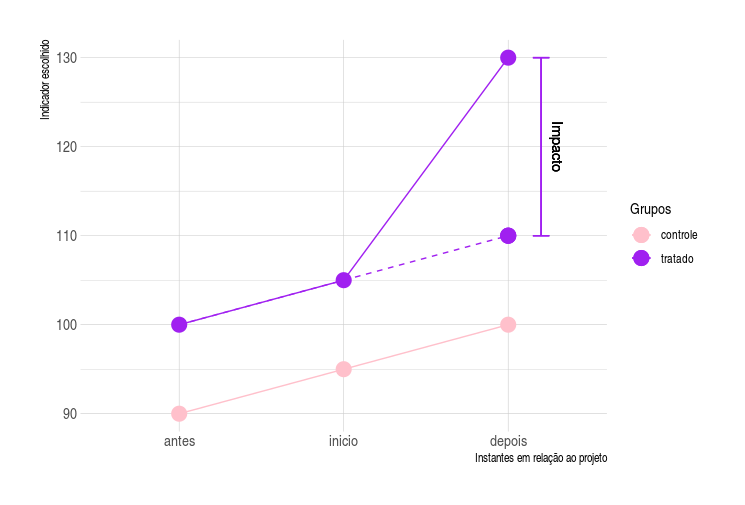
\includegraphics{impacto01.png}

Representação da avaliação de impacto

\hypertarget{poesias-contribuiuxe7uxf5es-externas.}{%
\section{Poesias, contribuições externas.}\label{poesias-contribuiuxe7uxf5es-externas.}}

\hypertarget{apuxeandice}{%
\chapter*{Apêndice}\label{apuxeandice}}
\addcontentsline{toc}{chapter}{Apêndice}

  \bibliography{book.bib,packages.bib}

\end{document}
